\documentclass[11pt,a4paper]{article}
\usepackage[a4paper,margin=2.0cm]{geometry}
\usepackage[T1]{fontenc}
\usepackage{lmodern}
\usepackage{microtype}
\usepackage{booktabs,tabularx,array}
\usepackage{graphicx}
\usepackage{xcolor}
\usepackage[inline]{enumitem}
\usepackage{caption}
\usepackage[most]{tcolorbox}
\usepackage{hyperref}
\usepackage[nameinlink,capitalise]{cleveref}
\hypersetup{colorlinks=true,linkcolor=teal!70!black,urlcolor=teal!70!black}
\definecolor{newblue}{RGB}{41,107,219}
\newcommand{\file}[1]{\texttt{\detokenize{#1}}}
\newtcolorbox{warn}{colback=orange!8,colframe=orange!70!black,boxrule=0.5pt,arc=2pt,left=4pt,right=4pt,top=2pt,bottom=2pt}
\newcommand{\step}[3]{%
\medskip\noindent
\begin{minipage}[t]{0.5\linewidth}\vspace{0pt}\centering
\includegraphics[width=\linewidth]{figures/#1.jpg}
\end{minipage}\hfill
\begin{minipage}[t]{0.47\linewidth}\vspace{0pt}\small
\textbf{#2}
#3
\end{minipage}\par}

\title{Kaiku desk robot --- assembly guide (MVP)}
\author{Junction 2026 · hardware (owner A)}
\date{14 November 2026 · design: \file{hardware/cad/} (D30, D31, D35)}

\begin{document}
\maketitle

\noindent This guide builds the MVP: the printed \textbf{head} and \textbf{neck} on a \textbf{cardboard body}. The renders come
from \file{hardware/cad/assembly_guide.py}, which draws the same parametric model the parts were printed from
(\file{kaiku_cad.py}). In each step, the parts being added are \textcolor{newblue}{\textbf{blue}}, the parts already
fitted are grey, and the cardboard box is brown. Where this guide and a ground-truth file disagree, the ground truth
wins: pins and cables in \file{hardware/wiring.md}, sizes in \file{hardware/dimensions.md}, electronics in
\file{docs/kaiku_robot_electronics_specs.md}.

\begin{figure}[h]\centering
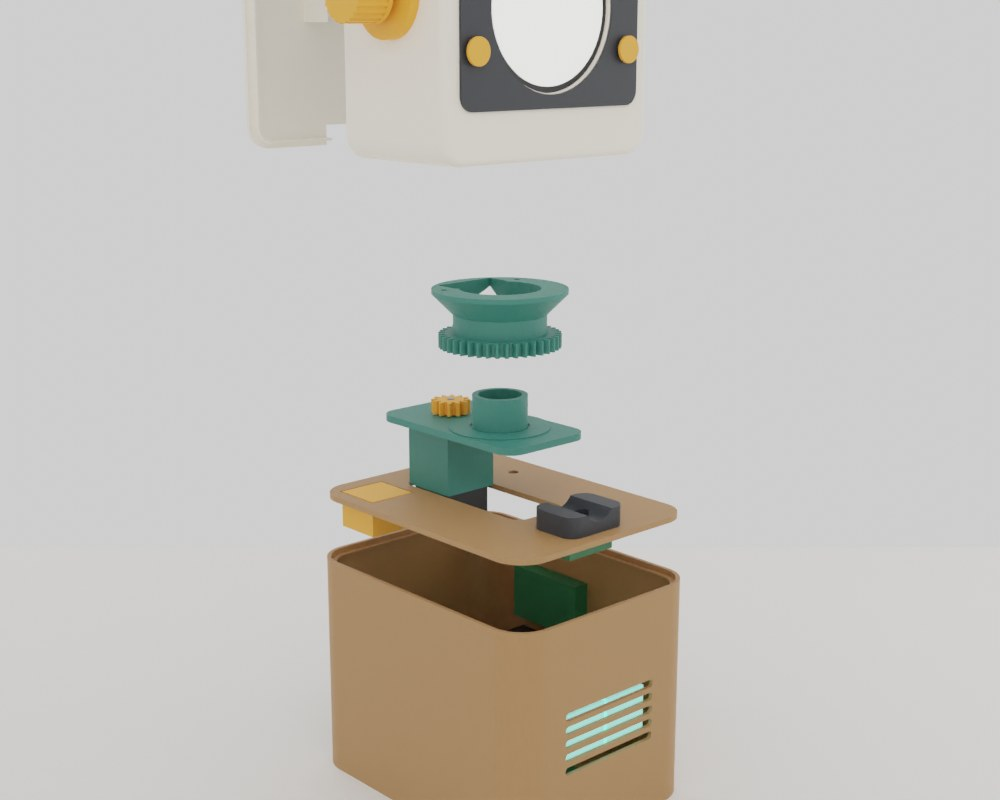
\includegraphics[width=0.62\linewidth]{figures/asm_0_exploded.jpg}
\caption{Exploded view: head, turntable, pan base with the pan motor, lid with the finger cradle, cardboard body.}
\end{figure}

\section{Before you start}

\paragraph{This build (D35).} One motor (pan). No hall sensor and no magnet: the head's \textbf{position at power-on is
``front''}, so always face it forward before plugging in. No light sensor: the camera measures room light. The
\file{purr_sleeve}, \file{purr_weight} and \file{window_pane} prints are not needed.

\paragraph{Printed parts.}
\begin{center}\small
\begin{tabularx}{\linewidth}{l l X}
\toprule
Part (\file{.stl}) & Plate & Used in\\
\midrule
\file{turntable}, \file{pan_base}, \file{pan_motor_mount}, \file{finger_cradle} & 2 (neck) & steps 1, 3--5, 15\\
\file{pinion}, \file{ear_left}, \file{ear_right}, \file{knob_cap}, \file{antenna_ball} & 3 (small) & steps 2, 8--10\\
\file{head_shell}, \file{head_back} & 1 (head) & steps 6--11, 13\\
\file{face_bezel}, \file{cheek_left}, \file{cheek_right} & 4 + 3 (optional) & step 12\\
\file{purr_sleeve}, \file{purr_weight}, \file{window_pane}, \file{body_tub}, \file{top_plate} & --- & not in the MVP\\
\bottomrule
\end{tabularx}
\end{center}

\paragraph{Bought-in parts.} Atech board with its USB-C module, Color Display, Knob, Button, Speaker, Microphone,
2 LED grids, 1 DC motor; Arduino UNO Q, USB camera (TPX00246), Modulino Buzzer, powered USB-C PD hub and the Arduino
power supply; KY-031, KY-039, KY-053; Atech cables and about 15 male--female jumpers, 30\,cm for the ones that go up
the neck.

\paragraph{Tools and consumables.} Hot-glue gun, superglue, double-sided foam tape, craft knife, steel ruler, flush
cutters, small pliers, 240-grit sandpaper, calipers; corrugated cardboard (about 500 $\times$ 300\,mm, 3--4\,mm
thick); tracing paper; a 3\,mm bamboo skewer or stiff wire for the antenna.

\begin{warn}
\textbf{Clean the prints first.} The parts were designed to print without supports, but some came off the printer
with support material. On the \file{turntable}: break out the support sheet in the middle and the rough band
between the gear and the disc. The rectangular \textbf{cable slot} must be fully open and the \textbf{centre hole}
clear. The ring-shaped \textbf{ledge} you see inside is real geometry (where the bore steps down onto the axle):
keep it. The \file{pan_motor_mount} must be an \textbf{open tube at both ends}.
\end{warn}

\paragraph{Test-fits before any glue.}
\begin{itemize}[leftmargin=1.2em]
\item \file{knob_cap}: a round $\approx$10\,mm bore (new version) slides over the Knob module's own black knob. A
small D-shaped hole is the old version: reprint \file{knob_cap.stl}.
\item The camera rests on its folded clip; check the clip folds flat under the body (about 64 $\times$ 37 $\times$
22\,mm).
\item The Color Display's screen should sit in the middle of the module's face (it did on the bench, within
$\pm$0.3\,mm).
\end{itemize}

\section{Neck}

\step{asm_1_testfit}{Step 1 -- test-fit the turntable on the pan base}{
\begin{enumerate}[leftmargin=1.2em]
\item Slide the \file{turntable}, gear side down, over the tube on the \file{pan_base}.
\item It should drop onto the thin ring on the base and spin with a tiny bit of play.
\item If it binds: sand the inside of the bore (not the tube) a little at a time. Never force it.
\end{enumerate}
\textbf{Check:} one full turn by hand, smooth and flat, with no rubbing on the gear teeth.}

\step{asm_2_pinion}{Step 2 -- pinion onto the pan motor}{
\begin{enumerate}[leftmargin=1.2em]
\item Find the flat on the motor's 3\,mm shaft and line up the pinion's D-hole with it.
\item Press the pinion on until its top face is \textbf{flush with the shaft end}.
\item Loose (round shaft or a sloppy print)? One drop of superglue on the shaft, none on the teeth.
\end{enumerate}
\textbf{Check:} the pinion runs true, with no wobble.}

\step{asm_3_sleeve}{Step 3 -- motor into its sleeve}{
\begin{enumerate}[leftmargin=1.2em]
\item Slide the motor into the open \file{pan_motor_mount} tube, shaft end first.
\item Stop when the motor's shaft-end face is flush with the tube's top edge. The connector end hangs out of the
bottom, with room for the cable plug.
\item Too loose? Add a strip of tape around the motor.
\end{enumerate}
\textbf{Check:} the end face is flush; the motor doesn't slide when you tip it.}

\step{asm_4_neck}{Step 4 -- mount the motor under the pan base, gears meshed}{
\begin{enumerate}[leftmargin=1.2em]
\item Put the turntable on the axle (step 1).
\item Hold the sleeve under the pan base so the pinion comes up through the small \O7 hole and meshes fully with the
ring gear, \textbf{with a hair of backlash}: the turntable should wiggle very slightly.
\item Keeping that mesh, superglue the sleeve's top edge to the underside of the flange. Then run a hot-glue fillet
all round (it carries the motor's torque).
\end{enumerate}
\textbf{Check:} teeth engaged over their full height; no binding. The real test is the motor bench run later.}

\step{asm_5_neck_on_lid}{Step 5 -- neck onto the cardboard lid}{
\begin{enumerate}[leftmargin=1.2em]
\item Cut the lid (104 $\times$ 136\,mm) and its pan hole (29 $\times$ 76\,mm, centred at 52\,mm from the left and
79\,mm from the front edge; \cref{sec:box}).
\item Drop the motor sleeve through the hole. The flange sits on top of the lid, the pinion towards the
\textbf{back}.
\item Hot-glue the flange to the lid all round.
\end{enumerate}
\textbf{Check:} the flange sits flat and the motor hangs straight down.}

\section{Head}

\step{asm_6_display}{Step 6 -- Color Display (the eyes)}{
\begin{enumerate}[leftmargin=1.2em]
\item Put the display into the frame behind the small window, \textbf{screen forward and connector edge up}: the
frame is open at the top for the cable plugs.
\item Check from the front that the screen fills the window, then tape the module's edges (never over the screen).
\end{enumerate}
\textbf{Check:} screen centred in the 28 $\times$ 13\,mm window; the plug edge has $\approx$12\,mm free above.}

\step{asm_7_camera}{Step 7 -- camera}{
\begin{enumerate}[leftmargin=1.2em]
\item Fold the camera's clip flat under its body.
\item Stand it on the head floor, ring light forward, and push it forward until its rim rests on the round lip.
\item Lead its USB cable back and down through the rectangular slot at the back of the floor.
\end{enumerate}
\textbf{Check:} the ring is centred in the \O65 opening. Too low: shim under the clip with cardboard.}

\step{asm_8_knob_ear}{Step 8 -- Knob (left ear)}{
\begin{enumerate}[leftmargin=1.2em]
\item Lay the square Knob module flat against the left inner wall, its knob out through the \O12 hole.
\item Glue the \file{ear_left} ring on the outside, centred on the knob.
\item Press the \file{knob_cap} over the module's black knob (a drop of glue if loose).
\item Optional: open the ear hole to $\approx$\O26 so the knob's light ring glows through.
\end{enumerate}
\textbf{Check:} the knob turns and clicks freely; the cap doesn't rub the ear ring.}

\step{asm_9_mic_ear}{Step 9 -- Microphone (right ear)}{
\begin{enumerate}[leftmargin=1.2em]
\item Put the Microphone module against the right inner wall, the face with its sound hole against the small holes.
\item Glue the \file{ear_right} grille on the outside, holes lined up.
\end{enumerate}
\textbf{Check:} nothing covers the holes from inside. (The mic is fitted but unused in v1.)}

\step{asm_10_knock_antenna}{Step 10 -- knock sensor and antenna}{
\begin{enumerate}[leftmargin=1.2em]
\item Stick the KY-031 flat under the head top, behind the display, on foam tape (taps reach the spring through it).
\item Connect three 30\,cm jumpers to S, + and $-$.
\item Push a 3\,mm skewer about 50\,mm long into the antenna socket on top (glue) and fit the \file{antenna_ball}.
\end{enumerate}
\textbf{Check:} a firm tap on the head top clicks the sensor.}

\step{asm_11_back_lid}{Step 11 -- cables, then the back lid}{
\begin{enumerate}[leftmargin=1.2em]
\item Plug in every head cable: display $\times$2, knob $\times$2, mic $\times$2, the three KY-031 jumpers, and the
camera USB. Route them all down through the floor slot.
\item Fit the \file{head_back}: its lip goes inside the opening, and its two ribs push the camera forward against
the lip. Tape it if it's loose.
\end{enumerate}
\textbf{Check:} the lid closes flush over the cable bundle (it has a notch at the bottom).}

\step{asm_12_face}{Step 12 -- face plate and cheeks (optional)}{
\begin{enumerate}[leftmargin=1.2em]
\item Glue the \file{face_bezel} on the front, centred on the ring and the window.
\item Glue the two cheeks below and beside the ring.
\end{enumerate}
\textbf{Check:} the bezel doesn't cover the ring light or the screen.}

\step{asm_13_head_on_neck}{Step 13 -- head onto the turntable}{
\begin{enumerate}[leftmargin=1.2em]
\item Feed the cable bundle down through the turntable's slot and the hollow axle, \textbf{camera USB-A plug
first}, then the rest one at a time.
\item Glue the head floor onto the turntable disc, \textbf{slot over slot}, head facing the front (away from the
pinion). Two M3 screws through the disc's holes are optional.
\item Leave a service loop of cable inside the body.
\end{enumerate}
\textbf{Check:} turning the head $\pm$80\textdegree{} by hand doesn't pull any cable.}

\section{Body (cardboard) and electronics}
\label{sec:box}

\paragraph{Cut list} (4\,mm board; positions are hole centres, measured from the panel's bottom-left corner as seen
from outside; 1:1 templates: \file{uv run --script hardware/cad/cardboard.py --t 4}).
\begin{center}\small
\begin{tabularx}{\linewidth}{l l X}
\toprule
Panel & Size (mm) & Cut-outs\\
\midrule
Bottom & 104 $\times$ 136 & none\\
Front & 104 $\times$ 92 & chest window 52 $\times$ 30 at (52, 43); tracing paper behind it\\
Back & 104 $\times$ 92 & cable slot 72 $\times$ 20 at (62, 11); Atech USB-C 18 $\times$ 14 at (84, 55)\\
Left & 128 $\times$ 92 & none (the Atech board is taped inside)\\
Right & 128 $\times$ 92 & speaker grille: 7 $\times$ 5 holes \O3, 6\,mm apart, the first at (60, 8)\\
Lid & 104 $\times$ 136 & pan hole 29 $\times$ 76 at (52, 79); button 23.4 square at (20, 114); pulse \O9 at
(52, 20); lift hole \O16 at (84, 120)\\
\bottomrule
\end{tabularx}
\end{center}
Glue the front and back standing on the bottom, then the two sides between them. Four cardboard strips glued under
the lid, 4\,mm in from its edges, keep it in place but removable.

\step{asm_14_body}{Step 14 -- electronics in the box}{
\begin{enumerate}[leftmargin=1.2em]
\item \textbf{Atech board} on the left wall, on a foam-tape stack about 8\,mm thick, USB-C module at the rear top
(lined up with the back hole).
\item \textbf{UNO Q} flat on the floor at the rear, USB-C facing the cable slot.
\item \textbf{Speaker} against the right wall behind the grille; \textbf{Modulino Buzzer} on the same wall above it.
\item \textbf{KY-053} on the floor in front of the UNO Q; \textbf{LED grids} behind the chest window, lit face
forward.
\item Wire everything as in \file{hardware/wiring.md} (summary in \cref{sec:wiring}).
\end{enumerate}
\textbf{Check:} nothing touches the motor's swing area under the lid.}

\step{asm_15_lid_parts}{Step 15 -- lid: pulse sensor and button}{
\begin{enumerate}[leftmargin=1.2em]
\item Tape the KY-039 under the \O9 hole, LED and sensor facing up.
\item Glue the \file{finger_cradle} on top, its hole over the \O9 hole, groove front-to-back.
\item Drop the Button module into its square hole.
\end{enumerate}
\textbf{Check:} a fingertip in the groove covers the sensor and blocks room light.}

\begin{figure}[h]\centering
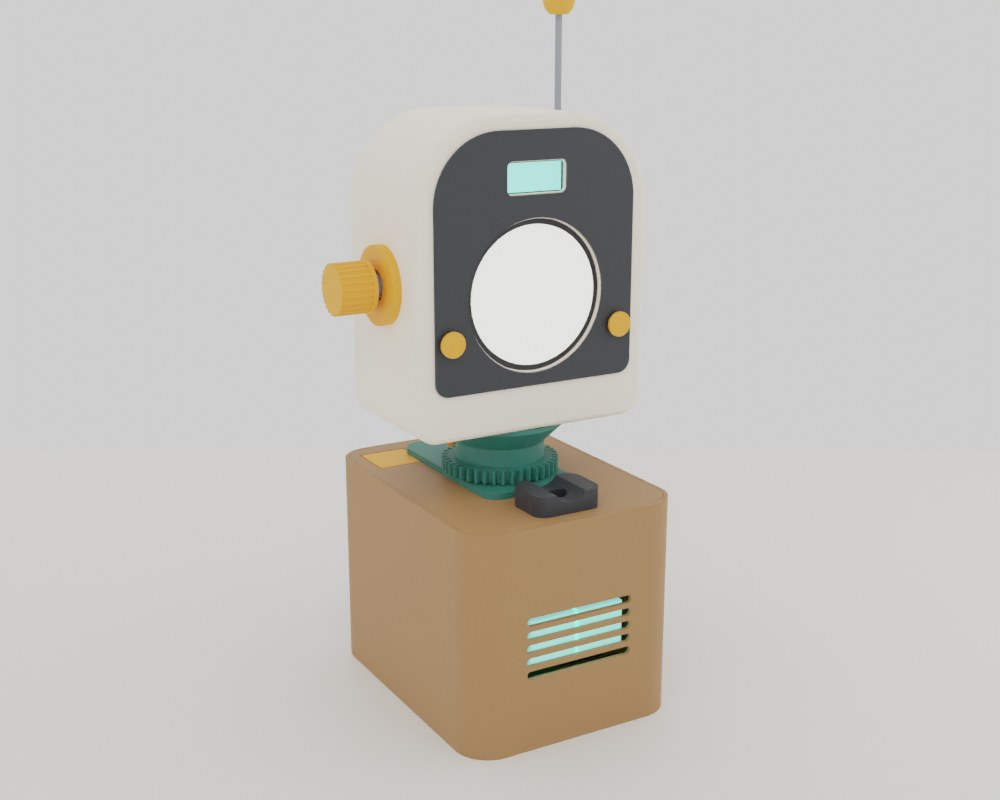
\includegraphics[width=0.55\linewidth]{figures/asm_16_complete.jpg}
\caption{The finished MVP.}
\end{figure}

\section{Wiring summary}
\label{sec:wiring}
Ground truth: \file{hardware/wiring.md}. Everything on the UNO Q is \textbf{3.3\,V}; never 5\,V. Unplug USB before
moving any wire.
\begin{center}\small
\begin{tabularx}{\linewidth}{>{\raggedright}p{0.27\linewidth} >{\raggedright}p{0.33\linewidth} X}
\toprule
From & To & Note\\
\midrule
Arduino supply & powered hub, PD input & the hub's fixed cable goes to the UNO Q\\
USB camera & a \emph{data} USB-A port on the hub & one port on our hub only charges\\
KY-031 S / + / $-$ & UNO Q D2 / 3.3V / GND & three 30\,cm jumpers up the neck\\
KY-053 SDA / SCL / VDD / GND & UNO Q SDA / SCL (by AREF) / 3.3V / GND & not A4/A5\\
KY-039 S / + / $-$ & KY-053 A0 / 3.3V / GND & \\
Modulino Buzzer & UNO Q Qwiic & \texttt{Wire1}, address 0x1E\\
Speaker / Display / Knob & Atech ports 1--2 / 3--4 / 5--6 & \\
Button / Mic & Atech ports 7 / 9--10 & \\
LED grids left / right & Atech ports 11 / 14 & port 11 stayed dark on the bench\\
Pan motor & Atech port 13 & \\
Atech power & Atech port 8 (USB-C module) & a data cable for flashing\\
\bottomrule
\end{tabularx}
\end{center}

\section{Before first power-on}
\begin{enumerate}[leftmargin=1.2em]
\item \textbf{Face the head forward.} That position becomes 0\textdegree; the firmware limits the head to
$\pm$80\textdegree{} from it.
\item Turn the head by hand through its range once more: no cable pulls.
\item Check every KY ``+'' goes to 3.3\,V, and that no bare jumper end touches anything.
\item Power the hub, then wait for the UNO Q's start-up animation to finish before plugging in the Atech board.
\item Run the bench tests part by part (\file{make bench-list}; \file{firmware/*/AGENTS.md}), starting with the pan
motor: it must turn the head both ways smoothly.
\end{enumerate}

\end{document}
